
\documentclass[12pt]{article}
\usepackage[utf8]{inputenc}
\usepackage{amsmath}
\usepackage{graphicx}
\usepackage{listings}
\setlength{\parskip}{\baselineskip}%
\setlength{\parindent}{0pt}%

\title{Computational Complexity Assignment 1}

\author{Tyler Tracy}

\begin{document}

\maketitle


\section{Problem 1}


The goal of this turing machine is to use a 3 tape turing machine to detect if a string is a palindrome.

My basic approach was to reverse the input string onto the second tape and then compare the first and second tape to see if they are the same.

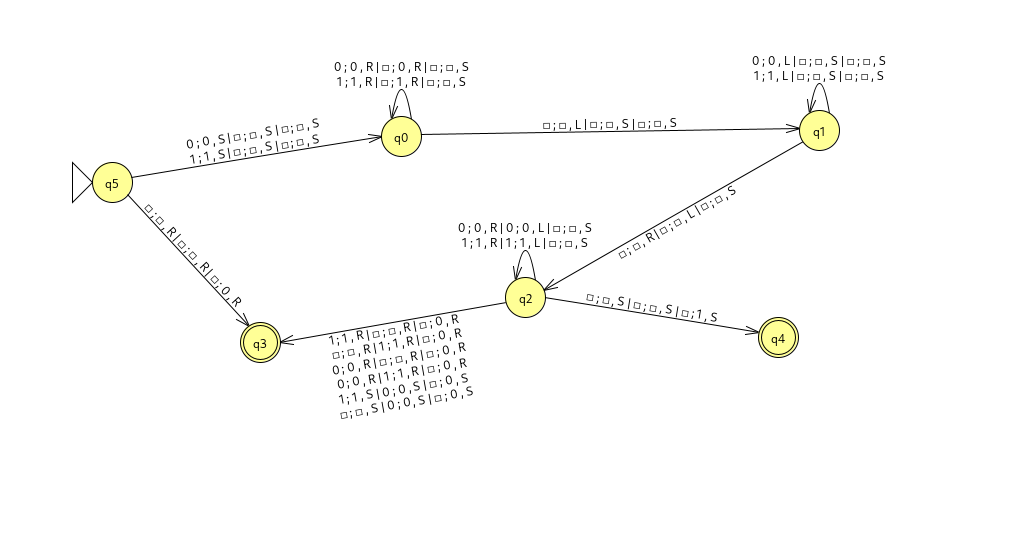
\includegraphics[width=\textwidth]{problem1.png}

Below I provide pseudocode for the turing machine and an analysis of the time complexity of each line

\begin{lstlisting}[basicstyle=\small, tabsize=3]
# Check for empty strings
If symbol under the first head is empty then reject # O(1)
# Move the head to the end of the input,
# Copying the string to the second tape
While first head is under a non-empty symbol # O(n)
	Move first head right # O(1)
	Write the symbol under the first head to the second tape # O(1)

# Move the first head back
While first head is under a non-empty symbol # O(n)
	Move the first head left # O(1)

# Compare the two strings
While first head is under a non-empty symbol # O(n)
	If the symbol under the first head is not the same
	as the symbol under the second head then reject # O(1)
	Move the first head right # O(1)
	Move the second head left # O(1)

accept
\end{lstlisting}

Adding all these complexities up and dropping the constants we get $O(n)$ for the time complexity of the turing machine.


\section{Problem 2}
The purpose of this turing machine is to detect if a string is a palindrome using a single tape turing machine.

My basic approach was to go back and forth between the beginning and end of the string and compare the characters at each end. If they are every different then the string is not a palindrome.

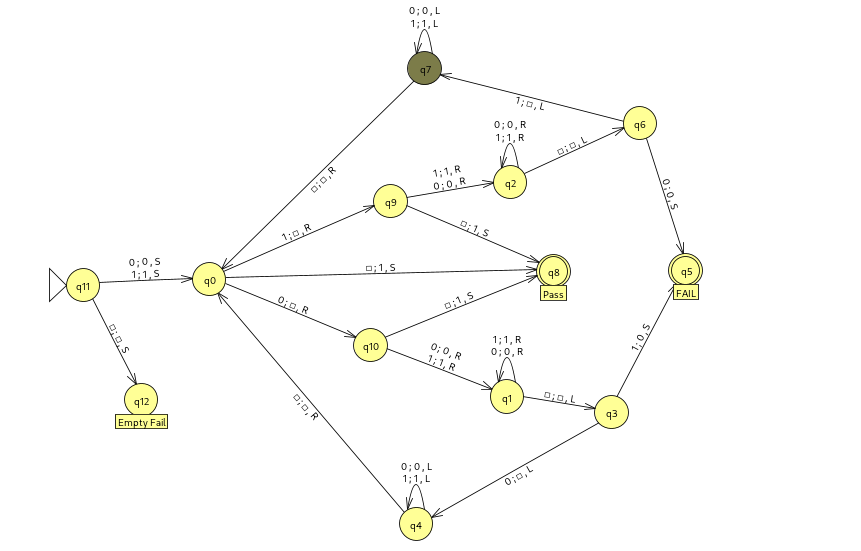
\includegraphics[width=\textwidth]{problem2.png}

Below I provide pseudocode for the turing machine and an analysis of the time complexity of each line

\begin{lstlisting}[basicstyle=\small, tabsize=2]
# Check for empty strings
If symbol under the head is empty then reject # O(1)

while the head is under a non-empty symbol # O(n)
	Store the symbol under the head in a variable i # O(1)
	Erase the symbol under the head # O(1)

	# Move the head to the end of the input
	While head is under a non-empty symbol # O(n)
		Move head right # O(1)
	Move the head left # O(1)

	If the symbol under the head is not the same as i
		then reject # O(1)

	# Move the head back to the beginning of the input
	While head is under a non-empty symbol # O(n)
		Move head left # O(1)
	Move head right # O(1)

accept
\end{lstlisting}

There are two nested loops in this program, the inner loop goes back and forth between across the string removing the ends, the outer loop loops over the inner until the the string is empty. Each of these loops are $O(n)$ so the total time complexity is $O(n^2)$.

\section{Problem 3}

My python program takes as input a jff file concatenated with an emoji and then the input. It splits the input across the emoji (which will not appear in the jff file or input) and then parse the jff file. JFF uses xml to encode the turing machine. XML is a very robust way to encode data, it trades space efficiency for robustness and readability. The jff file has lots of information in it but the only info that the python program needs is the transitions and the states. From the transitions, the tape alphabet and the input alphabet can be derived from all the symbols that appear. XML encodes an arbitrary amount of data by having starting and closing tags that surround data and put all data between those tags. The transitions and states are both encoded in this way so there can be as many of them as the turing machine needs.

To run the program run $./run.sh$ and to change the input change the $input.txt$ file.


\end{document}